\section{Rappresentazione degli insiemi}
\subsection{Diagrammi di Eulero-Venn}
Un metodo di rappresentazione grafico estremamente facile da capire ma limitato se si tratta di dover rappresentare insiemi grandi.
Molto semplicemente gli elementi dentro il cerchio appartengono all'insieme. \\
\begin{center}
    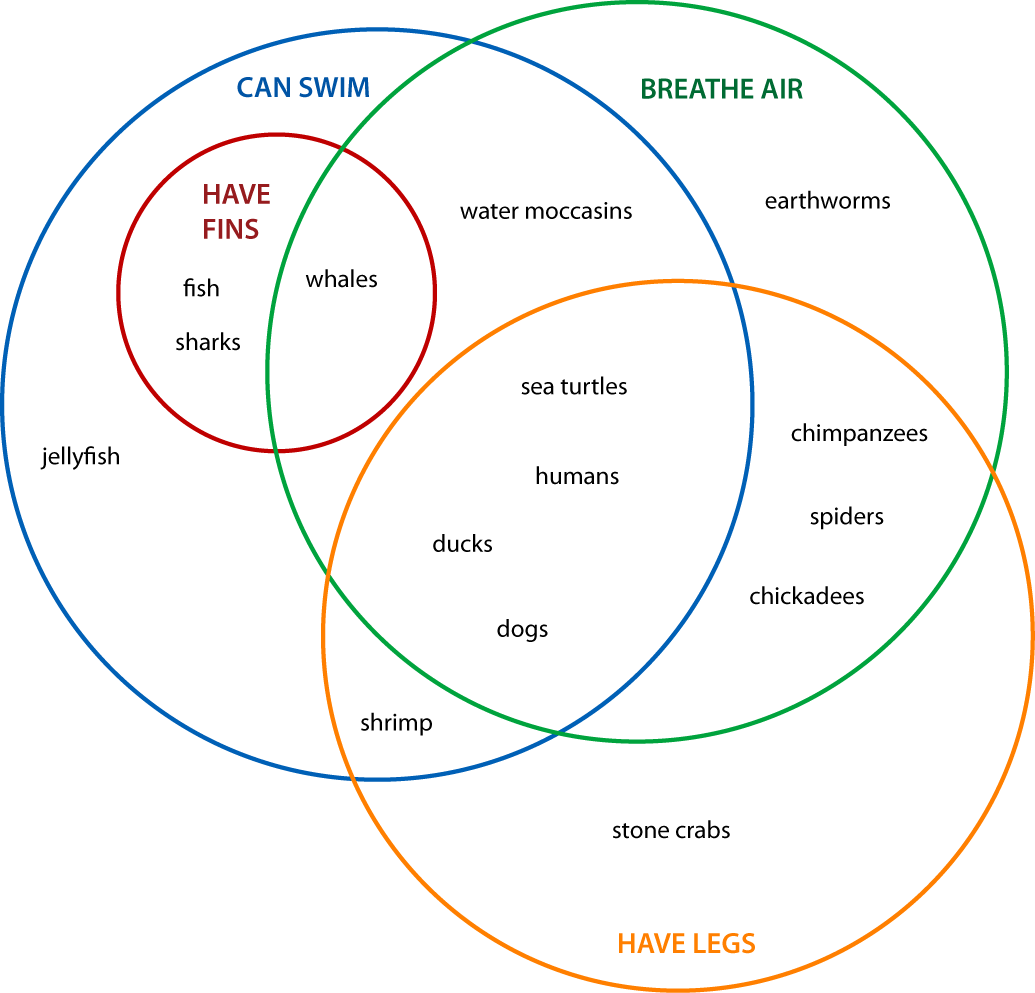
\includegraphics[scale=0.60]{Insiemi/venn-diagram1.png}
\end{center}

\subsection{Rappresentazione estensionale}
Consiste nell'elencare esplicitamente tutti gli elementi dell'insieme. \\
Anche questo metodo risulta scomodo quando all'interno dell'insieme vi è un gran numero
di elementi o addirittura c'è un numero infinito di elementi da elencare.
\begin{align*}
    &A = \{1, 2, 3\} \\
    &B = \{1, 2, 3, ..., 100\}
\end{align*}
\subsection{Rappresentazione intensionale}
Consiste nel formulare una proprietà caratteristica \textit{P} che distingue precisamente gli elementi dell'insieme S = \{x : \textit{P}\}. S è l'insieme di tutti e soli gli elementi per i quali la proprietà \textit{P} è vera. \\
\begin{center}
    A = \{x : x $\in$ $\mathbb{N}$, x $>$ 3, x $<$ 6\} = \{4, 5\}
\end{center}
